\section{Техническое задание}

\subsection{Основание для разработки}

Основанием для разработки является задание на выпускную квалификационную работу бакалавра «Разработка программно-информационной системы для организации и проведения занятий йогой», утверждённое приказом ректора ЮЗГУ от «16» апреля 2026 г. №1859-с. Разработка ведётся в соответствии с требованиями ГОСТ 34.602-89 «Техническое задание на создание автоматизированной системы».

\subsection{Цель и назначение разработки}

Программный продукт предназначен для автоматизации процесса записи клиентов на занятия йогой, управления расписанием и отслеживания прогресса пользователей. Целевой аудиторией приложения являются клиенты йога-студий, которые получают удобный инструмент для просмотра расписания, записи на занятия и отслеживания прогресса, а также администраторы и инструкторы, которые используют приложение для управления расписанием, просмотра записей и анализа загруженности.

\subsection{Требования к функциональности}

В таблице \ref{tab:func_req} приведён перечень функциональных требований к разрабатываемому приложению.

\renewcommand{\arraystretch}{1.3}
\begin{table}[H]
	\centering
	\caption{Функциональные требования}
	\label{tab:func_req}
	\normalsize
	\setlength{\tabcolsep}{6pt}
	\begin{tabular}{|m{3.8cm}|m{10cm}|}
		\hline
		\textbf{Идентификатор} & \textbf{Описание требования} \\
		\hline
		FR-01 & Авторизация пользователя с проверкой учётных данных \\
		\hline
		FR-02 & Регистрация нового пользователя (имя, email, пароль, уровень подготовки) \\
		\hline
		FR-03 & Просмотр каталога занятий с фильтрацией по городу \\
		\hline
		FR-04 & Просмотр детальной информации о занятии \\
		\hline
		FR-05 & Запись на выбранное занятие \\
		\hline
		FR-06 & Отмена существующей записи \\
		\hline
		FR-07 & Просмотр расписания с календарём на выбранную дату \\
		\hline
		FR-08 & Редактирование профиля пользователя (аватар, имя, email, город, уровень) \\
		\hline
		FR-09 & Просмотр списка инструкторов с фильтрацией по городу \\
		\hline
		FR-10 & Оставление отзыва и рейтинга (от 1 до 5 звёзд) \\
		\hline
		FR-11 & Просмотр статистики прогресса в виде графиков \\
		\hline
		FR-12 & Просмотр списка активных записей пользователя \\
		\hline
		FR-13 & Получение уведомления о записи на занятие \\
		\hline
		FR-14 & Получение напоминания о занятии за 1 час \\
		\hline
	\end{tabular}
\end{table}
\renewcommand{\arraystretch}{1}

\subsection{Нефункциональные требования}

В таблице \ref{tab:nonfunc_req} приведены нефункциональные требования к разрабатываемому приложению.

\renewcommand{\arraystretch}{1.3}
\begin{table}[H]
	\centering
	\caption{Нефункциональные требования}
	\label{tab:nonfunc_req}
	\normalsize
	\setlength{\tabcolsep}{6pt}
	\begin{tabular}{|m{4.5cm}|m{10cm}|}
		\hline
		\textbf{Категория} & \textbf{Описание требования} \\
		\hline
		Совместимость & Минимальная версия Android 7.0 (API level 24) \\
		\hline
		Локализация & Интерфейс на русском языке \\
		\hline
		Автономность & Работа без подключения к интернету (локальное хранение данных) \\
		\hline
		Производительность & Время отклика интерфейса не более 1 секунды \\
		\hline
		Надёжность & Сохранение данных пользователя при перезапуске приложения \\
		\hline
		Удобство использования & Интуитивно понятная навигация \\
		\hline
		Безопасность & Пароли хранятся в зашифрованном виде \\
		\hline
		Масштабируемость & Возможность добавления новых типов занятий без изменения кода \\
		\hline
	\end{tabular}
\end{table}
\renewcommand{\arraystretch}{1}

\subsection{Требования к интерфейсу}

Приложение должно включать в себя следующие экраны и элементы: навигацию по разделам с помощью BottomNavigationView с пятью вкладками, экран авторизации и регистрации, главный экран с приветствием и рекомендациями, каталог занятий с фильтрацией по городу, экран детальной информации о занятии, расписание с календарём, экран инструкторов с фильтрацией по городу, профиль пользователя с аватаром и настройками, экран статистики с графиками, экран моих записей, а также экран отзывов.

Интерфейс должен быть выполнен в едином стиле с использованием компонентов Material Design, обеспечивающих интуитивно понятное взаимодействие. Все элементы управления должны быть подписаны на русском языке. Шрифты должны быть достаточно крупными для комфортного чтения на экранах с диагональю от 5 дюймов.

\subsection{Моделирование вариантов использования}

На рисунке \ref{fig:usecase} представлена диаграмма прецедентов, демонстрирующая функциональные возможности приложения для пользователя.

\begin{figure}[H]
	\centering
	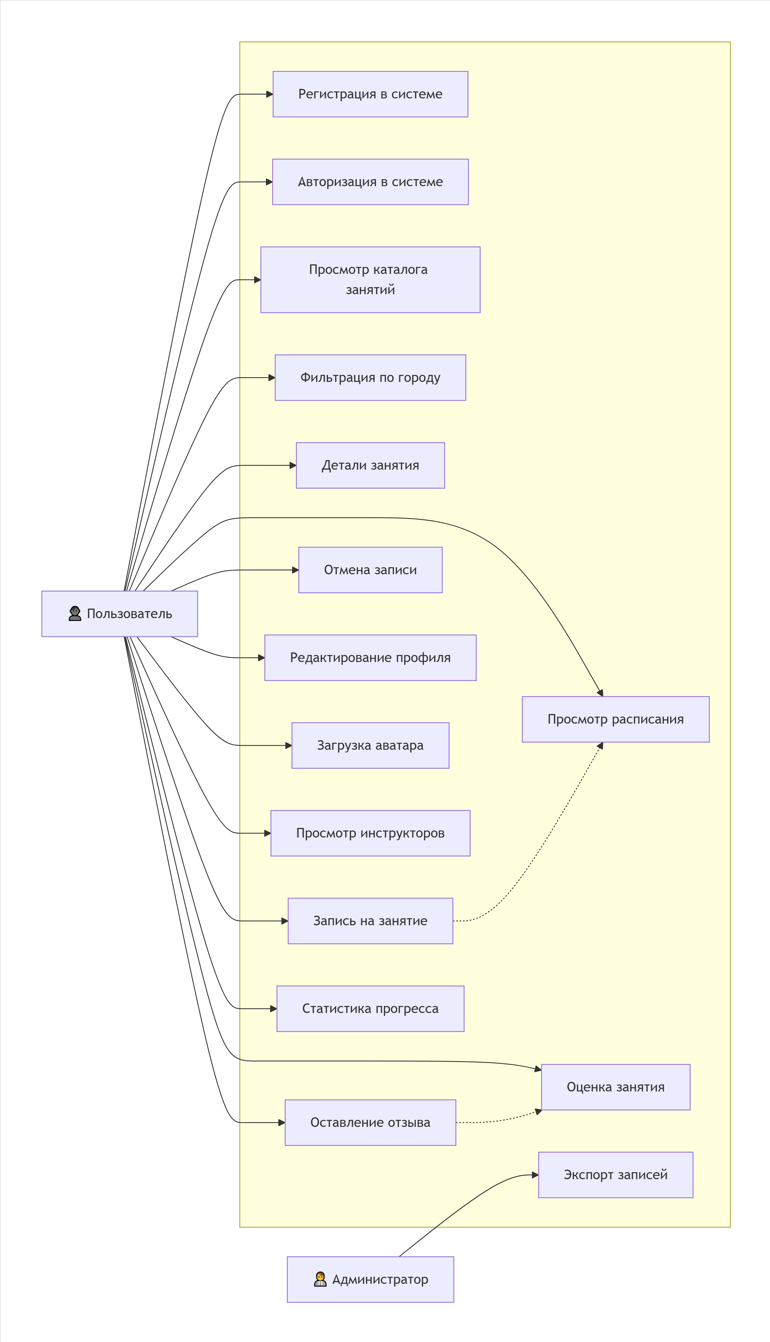
\includegraphics[width=0.8\textwidth]{images/use-case.png}
	\caption{Диаграмма прецедентов}
	\label{fig:usecase}
\end{figure}

Далее приведены агрегированные перечни прецедентов для каждой роли; они детализируются в последующих подпунктах.

\subsubsection{Вариант использования «Регистрация пользователя»}

\textbf{Предусловие:} приложение открыто на экране авторизации, пользователь не авторизован.

\textbf{Постусловие:} создана новая учётная запись, пользователь авторизован и перенаправлен на главный экран.

\textbf{Основной сценарий:}
\begin{enumerate}
	\item Пользователь нажимает кнопку «Регистрация».
	\item Система отображает форму регистрации.
	\item Пользователь вводит имя, адрес электронной почты, пароль и уровень подготовки.
	\item Пользователь нажимает кнопку «Зарегистрироваться».
	\item Система проверяет, не зарегистрирован ли уже указанный email.
	\item Если email свободен, система сохраняет данные в SharedPreferences.
	\item Система автоматически выполняет вход и открывает главный экран.
\end{enumerate}

\textbf{Альтернативный сценарий A1 (email уже зарегистрирован):}
\begin{enumerate}
	\item Система обнаруживает, что указанный email уже существует.
	\item Система отображает сообщение «Пользователь с таким email уже существует».
	\item Регистрация не выполняется, форма остаётся открытой.
\end{enumerate}

\textbf{Альтернативный сценарий A2 (не заполнены обязательные поля):}
\begin{enumerate}
	\item Система обнаруживает, что не все обязательные поля заполнены.
	\item Система подсвечивает незаполненные поля и отображает сообщение «Заполните все поля».
	\item Регистрация не выполняется.
\end{enumerate}

\subsubsection{Вариант использования «Авторизация пользователя»}

\textbf{Предусловие:} приложение открыто на экране авторизации, пользователь зарегистрирован.

\textbf{Постусловие:} пользователь авторизован и перенаправлен на главный экран.

\textbf{Основной сценарий:}
\begin{enumerate}
	\item Пользователь вводит адрес электронной почты и пароль.
	\item Пользователь нажимает кнопку «Войти».
	\item Система проверяет соответствие данных в SharedPreferences.
	\item Данные верны, система открывает главный экран.
\end{enumerate}

\textbf{Альтернативный сценарий A1 (неверный email или пароль):}
\begin{enumerate}
	\item Система проверяет данные и обнаруживает несоответствие.
	\item Система отображает сообщение «Неверный email или пароль».
	\item Пользователь остаётся на экране авторизации.
\end{enumerate}

\subsubsection{Вариант использования «Просмотр каталога занятий»}

\textbf{Предусловие:} пользователь авторизован, открыт главный экран.

\textbf{Постусловие:} отображён список доступных занятий.

\textbf{Основной сценарий:}
\begin{enumerate}
	\item Пользователь нажимает на вкладку «Занятия».
	\item Система загружает список занятий из SharedPreferences.
	\item Система отображает карточки занятий на экране.
	\item Пользователь просматривает список, прокручивая его.
\end{enumerate}

\textbf{Альтернативный сценарий A1 (список занятий пуст):}
\begin{enumerate}
	\item Система обнаруживает, что список занятий пуст.
	\item Система отображает сообщение «Нет доступных занятий».
\end{enumerate}

\subsubsection{Вариант использования «Фильтрация занятий по городу»}

\textbf{Предусловие:} открыт каталог занятий, список загружен.

\textbf{Постусловие:} отображаются только занятия выбранного города.

\textbf{Основной сценарий:}
\begin{enumerate}
	\item Пользователь нажимает на выпадающий список выбора города.
	\item Пользователь выбирает город (Москва, Санкт-Петербург или Казань).
	\item Система применяет фильтр к текущему набору занятий.
	\item Система обновляет карточки занятий на экране.
\end{enumerate}

\subsubsection{Вариант использования «Просмотр детальной информации о занятии»}

\textbf{Предусловие:} занятие отображается в списке или на карте.

\textbf{Постусловие:} открыт экран с детальной информацией о занятии.

\textbf{Основной сценарий:}
\begin{enumerate}
	\item Пользователь нажимает на карточку занятия в списке.
	\item Система открывает экран деталей.
	\item Система отображает название, описание, инструктора, время, место, цену и количество свободных мест.
\end{enumerate}

\subsubsection{Вариант использования «Запись на занятие»}

\textbf{Предусловие:} открыт экран детальной информации о занятии, пользователь не записан на это занятие.

\textbf{Постусловие:} запись сохранена, пользователь получает уведомление.

\textbf{Основной сценарий:}
\begin{enumerate}
	\item Пользователь нажимает кнопку «Записаться».
	\item Система проверяет наличие свободных мест.
	\item Места есть, система сохраняет запись в SharedPreferences.
	\item Система отправляет уведомление о подтверждении записи.
	\item Количество свободных мест уменьшается на 1.
\end{enumerate}

\textbf{Альтернативный сценарий A1 (нет свободных мест):}
\begin{enumerate}
	\item Система обнаруживает, что свободных мест нет.
	\item Система отображает сообщение «Нет свободных мест».
	\item Кнопка «Записаться» становится неактивной.
\end{enumerate}

\textbf{Альтернативный сценарий A2 (пользователь уже записан):}
\begin{enumerate}
	\item Система проверяет, не записан ли уже пользователь.
	\item Пользователь уже записан, система отображает сообщение «Вы уже записаны на это занятие».
\end{enumerate}

\subsubsection{Вариант использования «Отмена записи»}

\textbf{Предусловие:} пользователь записан на занятие, занятие ещё не началось.

\textbf{Постусловие:} запись удалена, место освобождено.

\textbf{Основной сценарий:}
\begin{enumerate}
	\item Пользователь открывает раздел «Мои записи».
	\item Пользователь выбирает запись для отмены.
	\item Пользователь нажимает кнопку «Отменить запись».
	\item Система удаляет запись из SharedPreferences.
	\item Система отображает сообщение «Запись отменена».
\end{enumerate}

\subsubsection{Вариант использования «Просмотр расписания с календарём»}

\textbf{Предусловие:} открыт раздел «Расписание».

\textbf{Постусловие:} отображены занятия на выбранную дату.

\textbf{Основной сценарий:}
\begin{enumerate}
	\item Пользователь открывает раздел «Расписание».
	\item Система отображает календарь на текущий месяц.
	\item Пользователь выбирает дату в календаре.
	\item Система фильтрует занятия по выбранной дате.
	\item Система отображает список занятий на выбранную дату.
\end{enumerate}

\subsubsection{Вариант использования «Просмотр списка инструкторов»}

\textbf{Предусловие:} открыт раздел «Инструкторы».

\textbf{Постусловие:} отображён список инструкторов.

\textbf{Основной сценарий:}
\begin{enumerate}
	\item Пользователь открывает раздел «Инструкторы».
	\item Система загружает список инструкторов из SharedPreferences.
	\item Система отображает карточки инструкторов на экране.
	\item При необходимости пользователь может отфильтровать инструкторов по городу.
\end{enumerate}

\subsubsection{Вариант использования «Редактирование профиля»}

\textbf{Предусловие:} открыт раздел «Профиль».

\textbf{Постусловие:} данные профиля обновлены.

\textbf{Основной сценарий:}
\begin{enumerate}
	\item Пользователь нажимает кнопку «Редактировать профиль».
	\item Система отображает форму с текущими данными.
	\item Пользователь изменяет нужные поля (аватар, имя, email, город, уровень подготовки).
	\item Пользователь нажимает кнопку «Сохранить».
	\item Система обновляет данные в SharedPreferences.
	\item Система отображает обновлённый профиль.
\end{enumerate}

\subsubsection{Вариант использования «Просмотр прогресса в виде графиков»}

\textbf{Предусловие:} открыт раздел «Прогресс».

\textbf{Постусловие:} отображены графики прогресса.

\textbf{Основной сценарий:}
\begin{enumerate}
	\item Пользователь открывает раздел «Прогресс».
	\item Система загружает данные о посещениях из SharedPreferences.
	\item Система строит графики (количество занятий по месяцам).
	\item Пользователь просматривает статистику.
	\item При необходимости пользователь может переключить отображаемый период (неделя, месяц, год).
\end{enumerate}

\subsubsection{Вариант использования «Оставление отзыва и рейтинга»}

\textbf{Предусловие:} занятие завершено, пользователь не оставлял отзыв ранее.

\textbf{Постусловие:} отзыв сохранён.

\textbf{Основной сценарий:}
\begin{enumerate}
	\item Пользователь открывает завершённое занятие в разделе «Мои записи».
	\item Пользователь нажимает кнопку «Оставить отзыв».
	\item Система отображает форму отзыва.
	\item Пользователь выбирает рейтинг от 1 до 5 звёзд.
	\item Пользователь вводит текстовый комментарий (опционально).
	\item Пользователь нажимает кнопку «Сохранить».
	\item Система сохраняет отзыв в SharedPreferences.
	\item Система обновляет рейтинг инструктора.
\end{enumerate}

\subsubsection{Вариант использования «Просмотр списка активных записей»}

\textbf{Предусловие:} открыт раздел «Мои записи».

\textbf{Постусловие:} отображены активные записи пользователя.

\textbf{Основной сценарий:}
\begin{enumerate}
	\item Пользователь открывает раздел «Мои записи».
	\item Система загружает записи из SharedPreferences.
	\item Система отображает список с указанием даты, времени, типа занятия и статуса.
	\item За один час до начала занятия система автоматически отправляет пользователю напоминание о предстоящем занятии.
\end{enumerate}

\subsection{Требования к надёжности}

Приложение должно корректно обрабатывать следующие аварийные ситуации: отсутствие свободного места на устройстве, прерывание работы приложения вследствие входящего звонка или сворачивания, а также некорректный ввод данных пользователем, при котором система должна показывать сообщения об ошибке. Все операции записи и изменения данных должны быть атомарными, что исключает частичное сохранение информации. Приложение должно восстанавливать состояние после принудительного закрытия.

\subsection{Требования к информационной безопасности}

Пароли пользователей должны храниться в зашифрованном виде с использованием стандартных механизмов Android. Все данные пользователя хранятся локально на устройстве и не передаются сторонним сервисам. Доступ к данным профиля осуществляется только через приложение. При некорректном вводе данных система не должна раскрывать информацию о существовании других пользователей. Приложение должно запрашивать только необходимые разрешения (доступ к хранилищу для аватара, доступ к уведомлениям).

\subsection{Требования к программной и технической совместимости}

Система должна корректно функционировать на устройствах под управлением операционной системы Android версии не ниже 7.0 (API level 24). Для работы приложения необходим установленный пакет Google Play Services. Клиентская часть не требует наличия дополнительного программного обеспечения. Рекомендуемый объём оперативной памяти устройства составляет не менее 2 ГБ. Приложение должно поддерживать экраны с разрешением от 480x800 до 1440x2960 пикселей.

\subsection{Требования к оформлению документации}

Разработка программной документации производится согласно ГОСТ 19.102-77 «Единая система программной документации. Стадии разработки», ГОСТ 34.601-90 «Информационная технология. Комплекс стандартов на автоматизированные системы. Стадии создания», а также СТУ 04.02.030-2017 «Курсовые работы (проекты). Выпускные квалификационные работы. Общие требования к структуре и оформлению».